We consider the case-study of vision-based lateral
control for a vehicle (explained in Section~\ref{sec:ch3_ProblemSetting}) for comparison of the three approaches
for control design with respect to the \gls{qoc} metrics described
earlier. The controllers for \gls{lqr} and switched linear control are tuned for the corresponding \gls{qoc} metric evaluation by adjusting the input and state weights. 

\subsection{Simulation results}
We illustrate an instance of our simulation that compares the three control paradigms: (i) for a reference output profile (for the control state $y_L$) shown in Fig.~\ref{fig:ch3_results} (a), we see that the \gls{slc} settles faster than both the \gls{mjls} and \gls{lqr} designs; and (ii) for control input shown in Fig.~\ref{fig:ch3_results} (b), we see that minimum control effort is needed for \gls{lqr}. \gls{slc} needs the highest control effort and might violate the input saturation requirements, if any. The control metrics \gls{psd} and \gls{mce} are derived from the control input $u[k]$ plots (e.g., see Fig.~\ref{fig:ch3_results}~(b)) and focus on minimizing the control effort or energy, whereas the control metrics \gls{mse} and \gls{st} are derived from the considered control output $y_L$ plots (e.g., see Fig.~\ref{fig:ch3_results}~(a)) and focus on improving the performance of the system output.  

We consider for the above simulation instance a frame rate of 30 fps, i.e., $\fh=\frac{1}{30}=33.33\ ms$ and an allocation of two processors. Then, we characterise the workload variations of a synthetic data set using a \gls{dtmc} model.
We notice that the $(h_i,\tau_i)$ for the worst-case workload $s_{wc}$ for this allocation is $(100,74)\ ms$. We then identify (as explained in Section \ref{sec:ch5_ch5_sys_scenario}) the three possible system scenarios $\{s_1=(\fh,33),\ s_2=(2\fh,57),\ s_3=s_{wc}=(3\fh,74)\}\ ms$. The transition probability matrix of the \gls{dtmc} model considered in this case for the three scenarios is: 
\begin{align}
P = 
\begin{bmatrix}
0.5 & 0.25 & 0.25 \\
0.25 & 0.5 & 0.25 \\
0.25 & 0.25 & 0.5 \nonumber
\end{bmatrix}.
\end{align}
The three controllers are then designed for the above scenarios as explained in Section~\ref{sec:ch3_control_design} using the input weight $d_u=1$. 

The control performance is then evaluated for the \gls{qoc} metrics (defined in Section~\ref{sec:ch3_control_problem}) - \gls{mse}, \gls{st}, \gls{psd}, \gls{mce} and combinations of \gls{mse}/\gls{st} with \gls{psd}/\gls{mce}. The combinations of \gls{mse}/\gls{st} with \gls{psd}/\gls{mce} is considered as they are contradictory in nature and optimising both together is a challenge and often times necessary.
% \scalebox{0.8}{
\begin{figure*}[t!]
    \centering
    \begin{subfigure}[t]{0.5\textwidth}
        \centering
        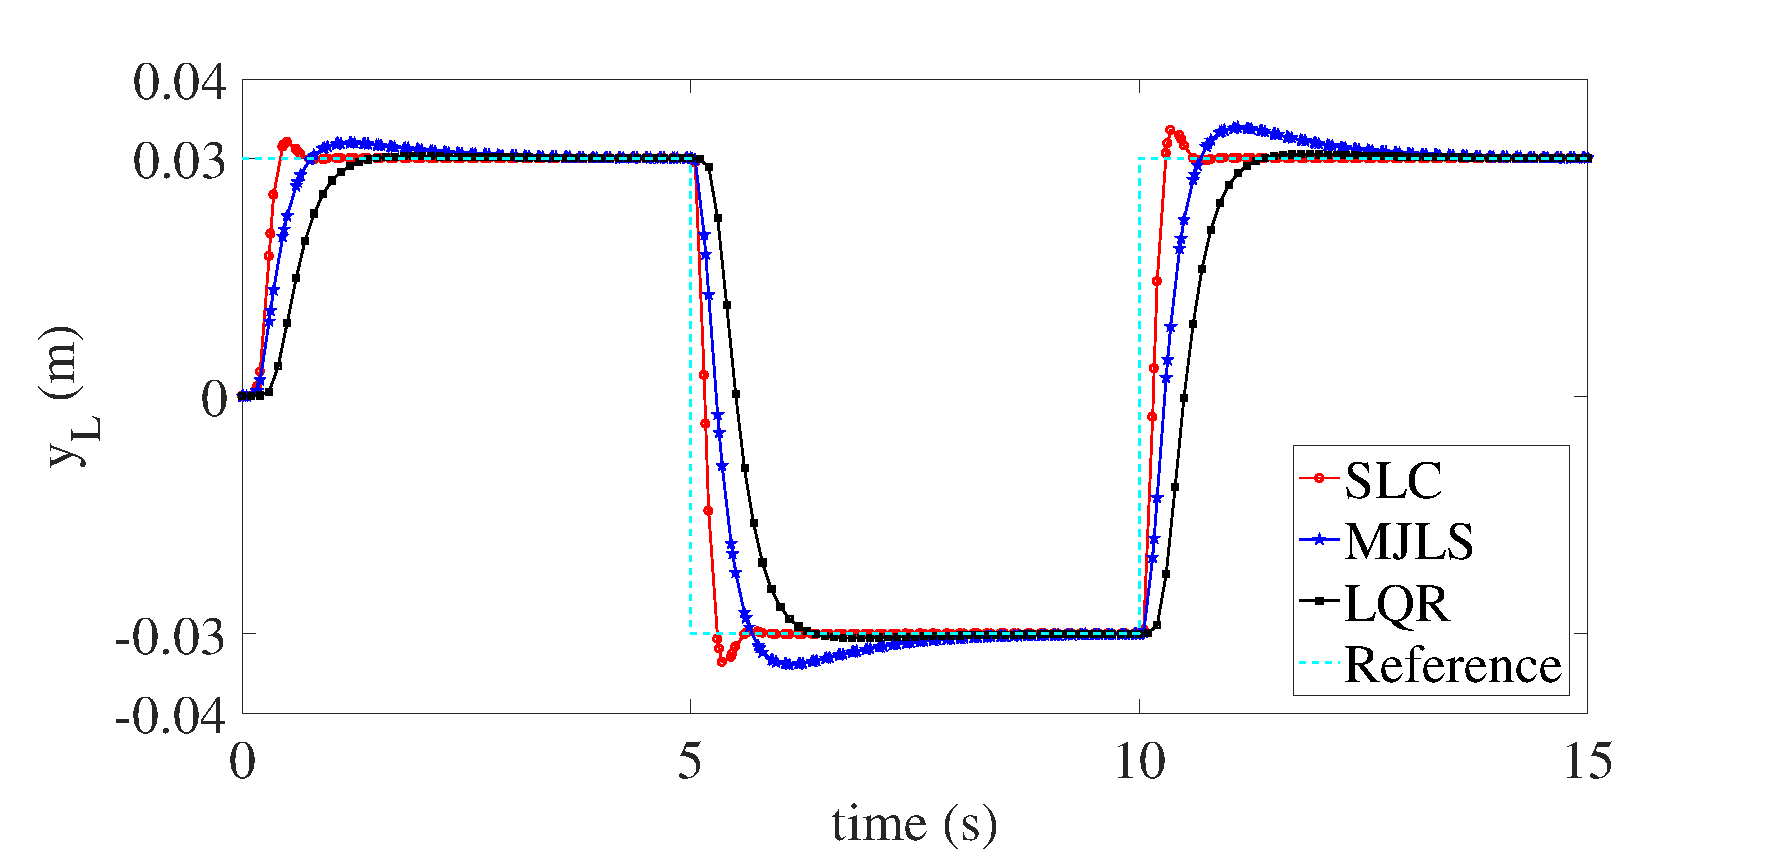
\includegraphics[width=\textwidth]{images/res_yL_R1.eps}
        \caption{Output $y_L$ when input weight $d_u=1$.}
    \end{subfigure}%
    ~ 
    \begin{subfigure}[t]{0.5\textwidth}
        \centering
       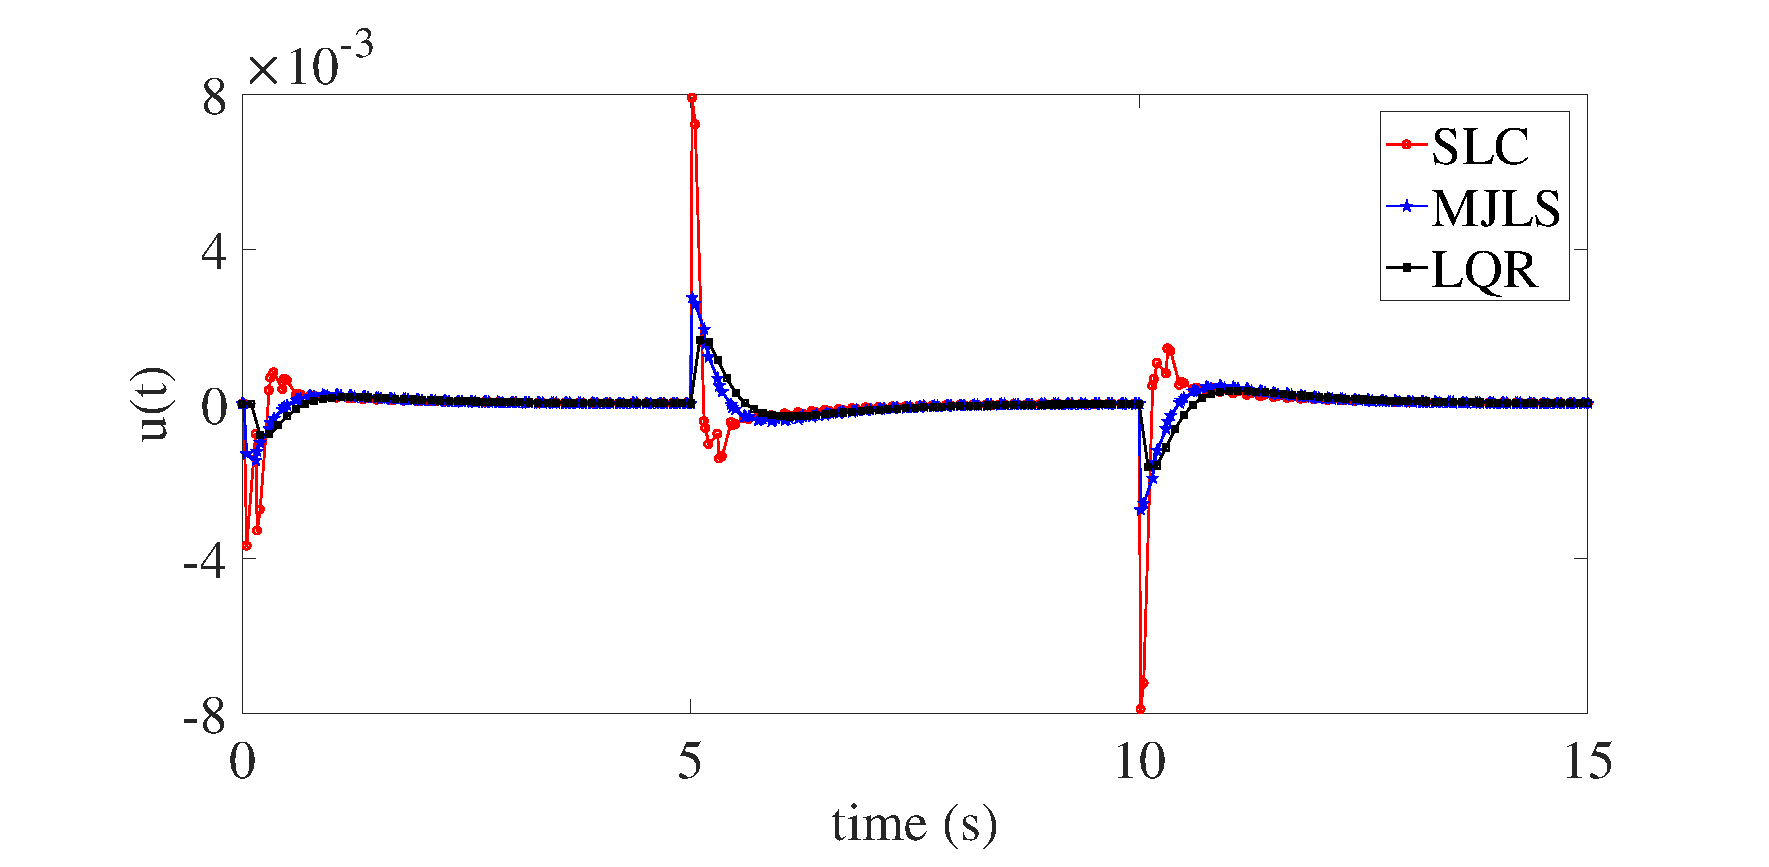
\includegraphics[width=\textwidth]{images/res_u_R1.eps}
       \caption{Input $u[k]$ when input weight $d_u=1$.}
    \end{subfigure}
    ~ 
    \begin{subfigure}[t]{0.5\textwidth}
        \centering
        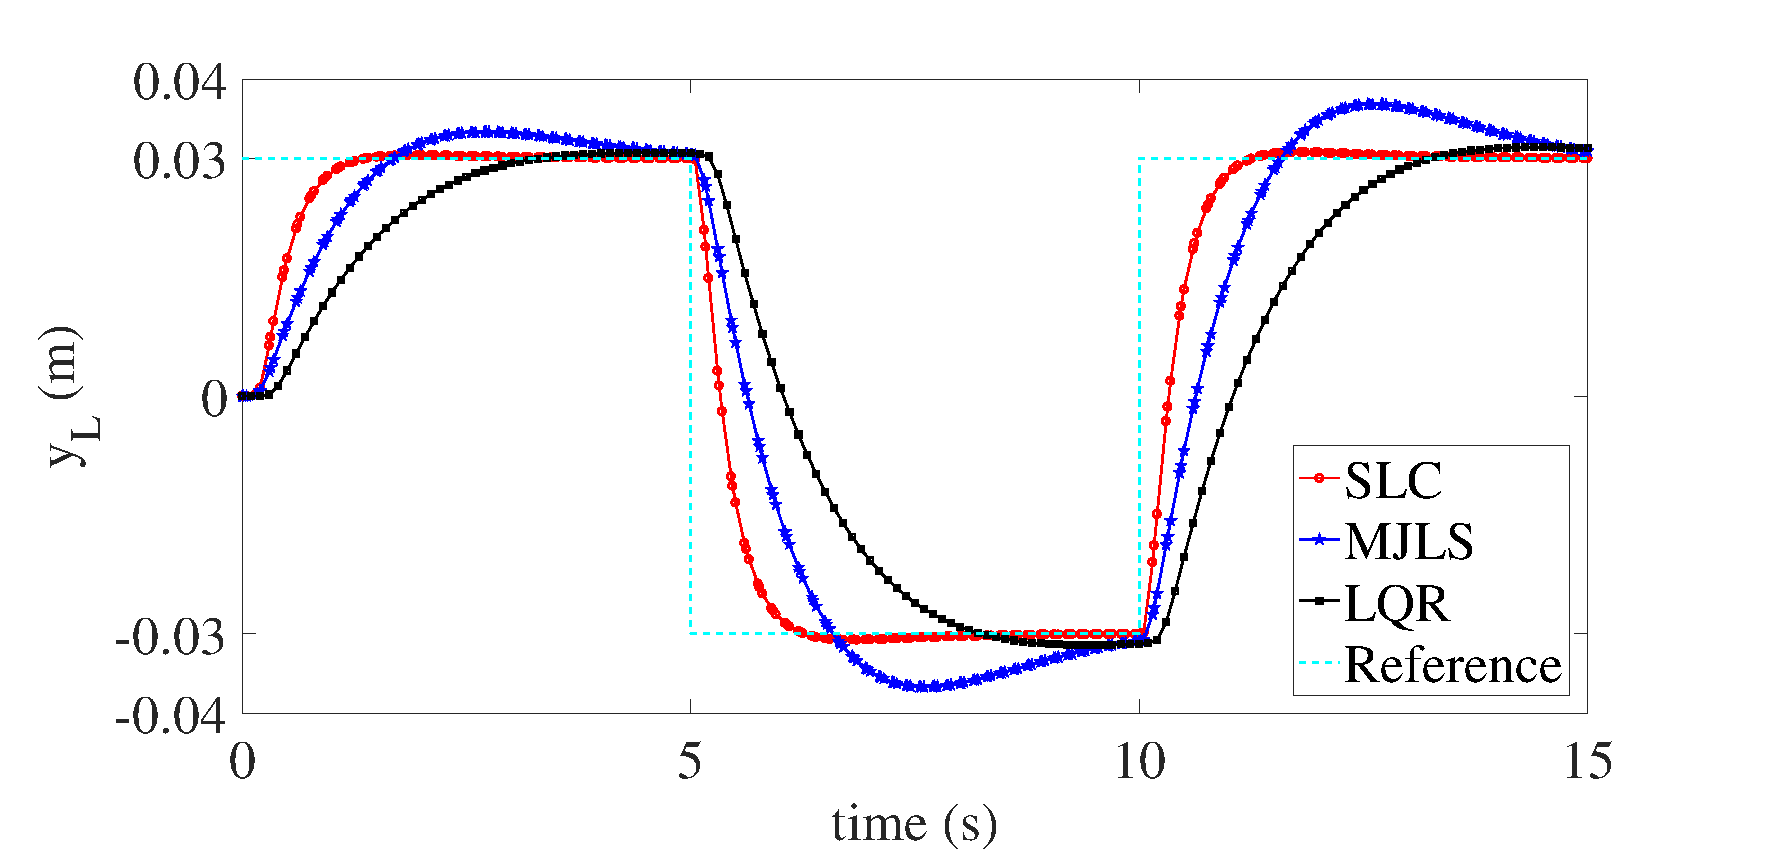
\includegraphics[width=\textwidth]{images/res_yL_R10.eps}
        \caption{Output $y_L$ when input weight $d_u=10$.}
    \end{subfigure}%
    ~
    \begin{subfigure}[t]{0.5\textwidth}
        \centering
       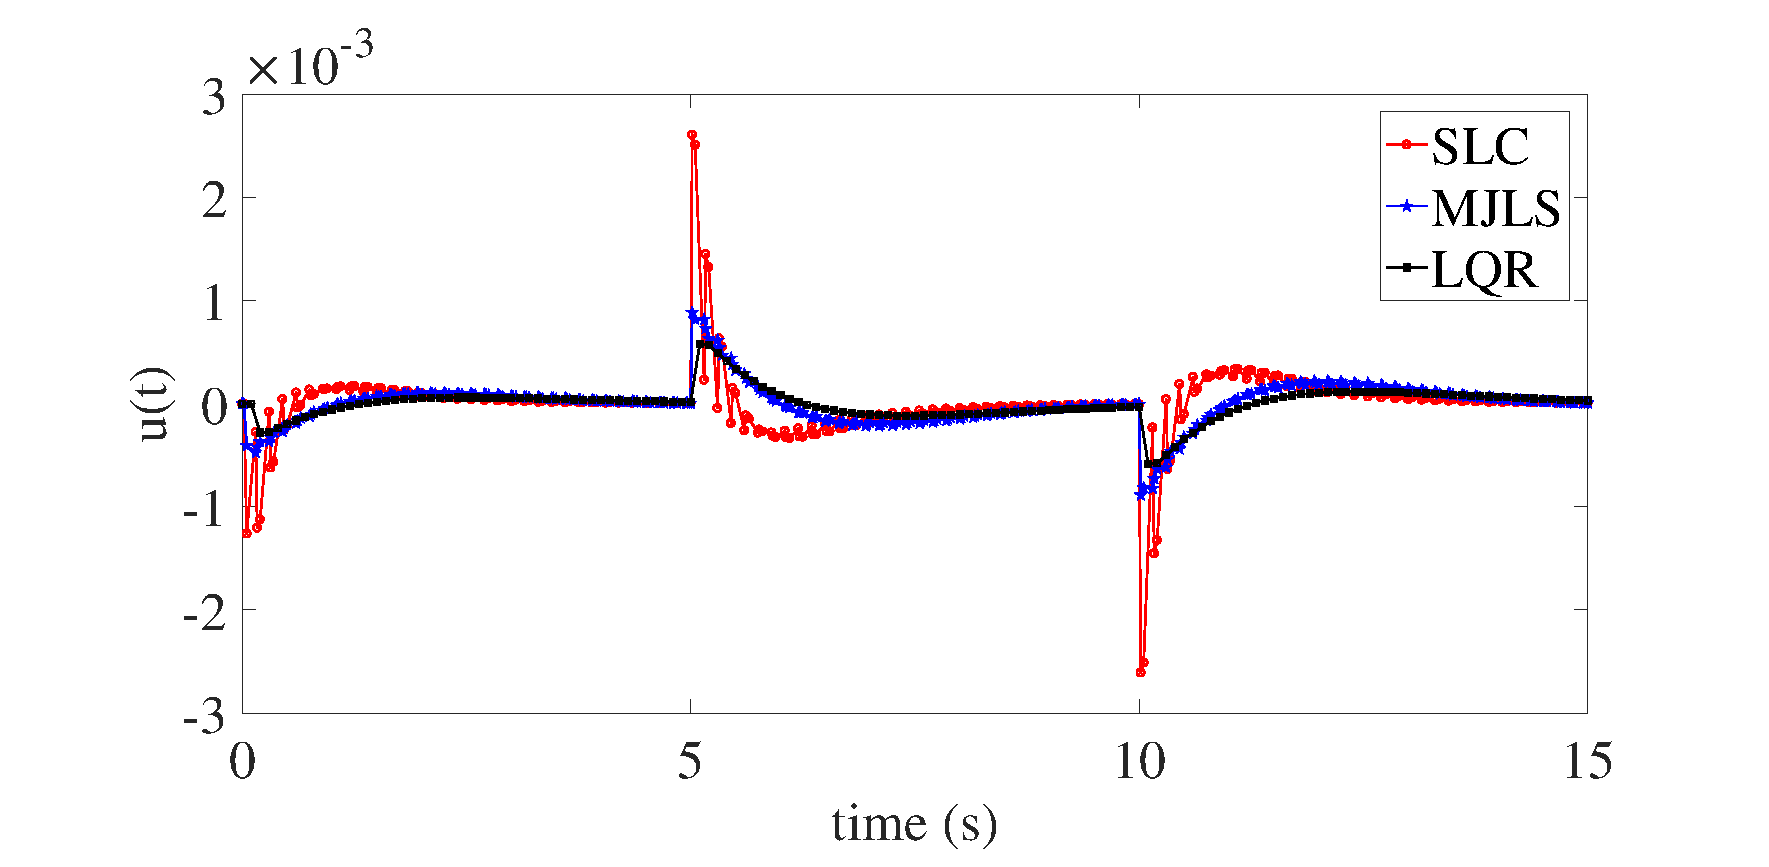
\includegraphics[width=\textwidth]{images/res_u_R10.eps}
       \caption{Input $u[k]$ when input weight $d_u=10$.}
    \end{subfigure}
    \caption{Comparison between controller synthesis method based on \gls{mjls} formulation (Section~\ref{sec:ch3_MJLS}), \gls{lqr} design (Section~\ref{sec:ch3_LQR}), and \gls{slc} system design (Section~\ref{sec:ch3_SPADe}). }
    \label{fig:ch3_results}
   \vspace{-2em}
\end{figure*}
% }
The above \gls{qoc} metrics' empirical cost for each control technique is evaluated over multiple runs of the simulation. Each simulation run generates different workload scenario sequences that satisfy the modelled \gls{dtmc}. These scenario sequences determine the switching sequence for both the \gls{slc} and \gls{mjls} control designs.


\subsection{Exploration and observations}
\label{sec:ch3_observations}
In order to provide design guidelines, we consider and vary the following different parameters: number of scenarios - we consider 3, 4 and 6 system scenarios; camera frame rates - 30 and 60 fps; input and state weights used for tuning the controllers; given platform allocation - 1, 2, 3, 4, 5, and 6 processors; and available system knowledge. We then evaluate the empirical cost of the \gls{qoc} metrics for each control technique over multiple runs of the simulation. The effects of varying these parameters are explained as follows:
\begin{enumerate}
    \item The number of states in the \gls{dtmc} model, the corresponding transition probability matrix and the number of control configurations change proportionally with the number of scenarios we consider. Only the \gls{slc} and \gls{mjls} system are affected by this parameter as the \gls{lqr} approach always (and only) considers the worst-case workload scenario;
    \item Changing the camera frame rate affects the total number of feasible scenarios we can have. As the maximum number of scenarios we can have, intuitively, is equal to $\lceil \frac{\tau_{wc}}{\fh}\rceil$, where $\tau_{wc}$ is the sensor-to-actuator delay for the worst-case workload (for a given platform allocation) and $\fh=\frac{1}{\text{camera fps}}$; 
    \item The input and state weights directly affect the control performance. E.g. for the simulation instance considered before, if we set the input weight $d_u=10$, we obtain the plots shown in Fig.~\ref{fig:ch3_results}~(c) and Fig.~\ref{fig:ch3_results}~(d). What we observe is a similar overall trend for the considered control paradigms. However, we see poorer \gls{qoc} metrics for \gls{mse} and \gls{st} and better \gls{qoc} metrics for \gls{psd} and \gls{mce}, when compared to $d_u=1$ and all other parameters remaining the same;
    \item The given platform allocation directly affects the timing parameters for a scenario $\workloadScenario$, i.e., $(h_i,\tau_i)$. A higher number of available processors mean that we could execute more tasks in parallel and reduce the  $(h_i,\tau_i)$ (even) for the worst-case workload scenario. This means that we could possibly reduce the total number of scenarios as well;
    \item System knowledge is an important parameter that determines which control design techniques can be used. An optimal control design using \gls{lqr} only requires the worst-case (workload) timing information. However,  designing an \gls{slc} system requires information regarding frequently occurring workloads as well and for the \gls{mjls} synthesis approach, we need both the frequently occurring workloads and their transition probabilities.
\end{enumerate}

\begin{table*}[t]
	\normalsize
	\begin{center}
\caption{Guidelines for choosing the control design techniques: MJLS (Section~\ref{sec:ch3_MJLS}), \gls{lqr} (Section~\ref{sec:ch3_LQR}), \gls{slc} (Section~\ref{sec:ch3_SPADe}).}
\label{Table:Results}
\scriptsize
\begin{tabular}{|c|c|c|c|c|c|}
\hline
\multirow{3}{*}{Available system knowledge}                                                                            & \multicolumn{5}{c|}{\gls{qoc} metrics}                                                                                                                                                                                                                                                                         \\ \cline{2-6} 
                                                                                                                       & \multicolumn{2}{c|}{Performance}                                                                        & \multicolumn{2}{c|}{Control energy}                                                                             & \multirow{2}{*}{\begin{tabular}[c]{@{}c@{}}Performance\\ and Energy\end{tabular}} \\ \cline{2-5}
                                                                                                                       & \gls{mse}                                                & \gls{st}                                                 & \gls{mce}                                                & \gls{psd}                                                &                                                                                      \\ \hline
Only worst-case workload information                                                                                   & \gls{lqr}                                                & \gls{lqr}                                                & \gls{lqr}                                                & \gls{lqr}                                                & \gls{lqr}                                                                                  \\ \hline
Frequently occurring workloads as a PERT                                                                               & \gls{slc}                                                & \gls{slc}                                                & \gls{lqr}                                                & \gls{lqr}                                                & \gls{slc}/ \gls{lqr}                                                                             \\ \hline
\begin{tabular}[c]{@{}c@{}}Frequently occurring workloads and their \\ transition probabilities as a \gls{dtmc}\end{tabular} & \begin{tabular}[c]{@{}c@{}}\gls{slc}/\\ MJLS\end{tabular} & \begin{tabular}[c]{@{}c@{}}\gls{slc}/\\ MJLS\end{tabular} & \begin{tabular}[c]{@{}c@{}}MJLS/\\ \gls{lqr}\end{tabular} & \begin{tabular}[c]{@{}c@{}}MJLS/\\ \gls{lqr}\end{tabular} & MJLS                                                                                  \\ \hline
\end{tabular}
\end{center}
%\horizontalEqSep
\vspace{-2em}
\end{table*}
\vspace{-0.5em}
\subsection{Design guidelines}
The design guidelines we have inferred from observing our simulations for choosing the control design techniques for different \gls{qoc} metrics and available system knowledge are listed in Table.~\ref{Table:Results}. The cases we see in the table are explained below.
\begin{itemize}
    \item \emph{Only worst-case workload information is known:}
    This situation is quite common for a control designer. Worst-case response time or delay of the algorithms can be analysed (where often times are pessimistic) through profiling and/or analytical methods~\cite{saidi2018future}. The control designer is then given only the worst-case timing information and is asked to design a controller with a \gls{qoc} requirement. In this case, the \gls{slc} and \gls{mjls} approach are not applicable and only the optimal \gls{lqr} design approach can be used. 
    
    \item \emph{PERT distribution is known:} Here, like we did in Chapters \ref{chap:parallelisation} and \ref{chap:pipelined_parallelism},  we assume that the information with respect to frequently occurring workloads is known and are characterised analytically as a PERT distribution~\cite{adyanthaya2014robustness}. In this case, \gls{slc} wins for performance-oriented metrics - \gls{mse} and \gls{st}, and \gls{lqr} wins for control effort or energy-oriented metrics - \gls{psd} and \gls{mce}. For jointly optimising performance and energy, there is no clear winner as it depends mainly on which of the two metrics is more important. If performance is important, \gls{slc} is preferred and if energy is important, \gls{lqr} should be chosen.
    The \gls{mjls} approach is not applicable as more information is needed.
    
    \item \emph{\gls{dtmc} model is known:} Information regarding frequently occurring workloads and their transition probabilities are needed for modelling a \gls{dtmc}. These can be estimated from observed workload-variations data~\cite{welton2005estimation}. Intuitively, this means that we can predict the possible (workload) scenario switching sequences for the control design. However, for the above two cases the switching sequence is assumed to be arbitrary and not known.  In this case, for performance metrics, \gls{mjls} wins when the input weight $d_u$ is very small (since \gls{slc} tends to oscillate before settling). However, for a large value of $d_u$, there is no clear winner between \gls{slc} and \gls{mjls} and it depends on the application and chosen parameters. Please note, however, that a challenge of \gls{slc} is to prove the stability of the designed system. \gls{mjls} is a synthesis method and the design, if any, is stable by construction.\\
          If we consider control effort or energy metrics, \gls{lqr} wins when the input weight $d_u$ is small and there is no clear winner between \gls{lqr} and \gls{mjls} for a large input weight $d_u$ as the results are similar and depend on the application and chosen parameters. \gls{mjls} is the clear winner if we consider a joint optimisation for performance and energy \gls{qoc} metrics.
\end{itemize}